\begin{figure}[!h]
  \centering
  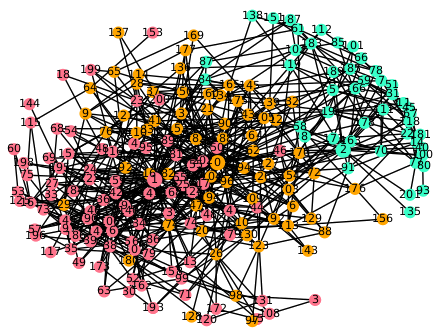
\includegraphics[trim={2.1cm 2cm 2cm 2cm}, clip, width=\columnwidth]{img/pdf/cover}
  \caption{Example of a simulation run with: sources: 3, users: 200, cycles:800, average degree: 5, seed: 123456789}
  \label{fig:abstract}
\end{figure}

\section*{Abstract}\label{abstract}
Our aim is to analyse the influence of memory in a news spreading dynamic. In order to do that, we have built a framework of agents 
connected in a network and equipped them with a set of basic functions. We wish to observe a diffusion-like process.
In this paper we expose the underlying methodology and try to explain it with a simple tutorial.

\section{Introduction}\label{sec:introduction}
For the purpose of modeling the interactions between users in the context of news spreading, it is convenient to talk about autonomous agents
linked by friendly ties whose overall view constitutes the network.
Network population is made of two breeds of agents: sources and users. These two breeds will interact
in an autonomous approach during program execution.
The network is initially a random connection of agents and modifies its own topology following a set of microscopic agents' actions.
\\In our opinion the interactions, due to natural news diffusion in a social-like network, are guided by news' feature to capture each agent's attention and by the agents social impact.
We hope to observe a spontaneous growth of scale-free regime starting from dynamical micro-interactions.\\ We also hope to reveal 
a natural segregation behaviour that subjugate a great deal of real social networks.
In addition to these items we wonder if there can be correlation between news spreading and agents' memory lenght.
From a technical point of view, we have worked with the Swarm-like protocol in python 3 named SLAPP.\footnote{For reference and download from: \url{https://github.com/terna/SLAPP}}

\section{Overview}\label{sec:overview}
We have built our model focusing on two coexisting points of view: agent based nature and network framework. 
We have blended these two frames considering a network of agents. 
\subsection{Context}
Let us focus on the dynamical process of rumor spreading in a social\footnote{The word \textit{social} can be thought in a general context.} network.
\\ News diffusion is generally studied in a stochastic context, ruled by a set of stochastic differential equations.
 There is an apparent similarity with epidemiological processes. 
However, while epidemic diffusion becomes a viral process when a threshold is exceeded, rumor spreading process seems to be threshold-less.
 The epidemic model of information diffusion is usually a compartmental model in which agents, in different stages, coexist in the world.
 Most of initial users stays in the compartment of \textit{ignorants} whereas a minority of them stays in the \textit{spreader} compartment.
 There is also another compartment, the \textit{stiflers}: users influenced by news who do not spread anymore (equivalent to \textit{recovery} in the SIR model.\footnote{Acronym of Susceptible-Infected-Recovery, most famous model of epidemic spreading. For more details, see for instance }).
\\ This \textit{Spreader-Ignorant-stifler} model (SIs) can be sketched by a set of transition between compartments; one of the transition is spontaneous while the others are induced by contact:
\begin{itemize}
\item$ I \longrightarrow S$
\item $S+I \longrightarrow S + S$

\item $S + S \longrightarrow s + S$

\item $s + S \longrightarrow  s + s$
\end{itemize}

$S$ is the Spreader status, $I$ is the Ignorant and $s$ the Stifler. 
The first process corresponds to the spontaneous transition from the ignorant compartment to spreader compartment;
 the second one corresponds to the contamination of an ignorant by contact with a spreader user; 
the third and fourth interactions reproduce transitions by contact to the Stifler compartment.
Development of dynamics is governed by sequences of users transitions from a compartment to another one, until all users which were spreaders reach the stifler compartment and the remaining ignorants stay in their compartment.\\
This approach is applicable to a network of users to predict the reproductive 
number\footnote{The reproductive number $R_{0}$ is defined by characteristic parameters that affect spreading like average degree (in first approximation) and diffusion rate. } 
which enable us to estimate the future qualitative behaviour of spreading: 
if this number is above some epidemic threshold then virality of diffusion is guaranteed.\\
This description can be reliable with a single viral diffusion of news, but when a
multiple news diffusion occurs, the analysis by a set of several differential equations would result more difficult.  
 \\ A compartmental approach to study the phenomenon of information diffusion has been widely examined in the last years, with very different variants of naive models CITAZIONIII.
There are also several papers underlining interesting results in social science: for example social influence, infection, segregation, homophily or fake news diffusion; or also the effects of fact-checking or bot-agent insertion in a network.
 In news spreading literature, only few models are built on an agent architecture and we report references in the bibliography.


\subsection{Why Agents?}\label{subsec:whyagents}
Agents are a very useful paradigm to model social interactions. 
They can operate in their environment, take decisions and interact with each other.
There is no communication protocol between them but they communicate and share news with "friends". \\
The environment is not deterministic. 
Every action can produce different effects with a different probability, but the simulation must be reproducible.
Actions between agents are non-deterministic. Agents don't have complete control of another agent; agents have limited senses and sensors.
\\
The required characteristics of each agent are: \begin{itemize}
\item [\textit {Rationality:}] agents can take choices depending on their own belief and their surrounding environment;
\item [\textit {reactivity:}] agents can check the World clock and news spreading nearby during the dynamic;
\item [\textit {proactiveness:}] agents can express their own will, taking autonomous initiatives;
\item [\textit {social Ability:}] They know how to send and receive news, to determine sympathy with neighbours;
\item [no \textit{mobility}] is required. 
\end{itemize}

Each agent can receive information from the world or from another agent; he can also interact with 
the world or with an agent, in order to meet its own character (a.k.a. state of mind).
They can modify their surrounding environment by means of the insertion or removal of a link in the social network.
The only accessible variable for each agent is the clock number; they can also access some neighbours' information.
\\
Each agent makes local fair decisions: global behaviours may emerge.
When active each agent can control the environment and reacts to the changes. 
It is possible that during his inactive state the environment has changed so the previous buffered action cannot be performed.
For this reason the agent can act unpredictably and somehow irrational.
